\section{Background}\label{sec:background}

TODO introduction
\subsection{Spark}\label{subsec:spark}
Spark is the probably most widely used and industry accepted cluster computing model.
It improves over former computing models, e.g. MapReduce~\cite{mapreduce}, Hadoop~\cite{hadoop} or Haloop~\cite{haloop},
by allowing to cache results in memory between multiple queries, using so-called resilient
distributed datasets~\cite{rdd}; often abbreviated to RDD.

This section introduces Spark and is organized in four subsections.
\Cref{subsubsec:resilient-distributed-datasets} describes the core data structure of Spark: the RDD's.
In~\cref{subsubsec:spark-architecture}, we explain the different components and processes in a Spark cluster.
The query optimizer of Spark, Catalyst, is explained in~\cref{subsubsec:catalyst}.
It is the component we integrate our \textsc{WCOJ} with;
therefore, it is the module of Spark that is most relevant to this thesis.
Finally, in~\cref{subsubsec:broadcast-variables} we highlight important details about \textit{Broadcast variables} which are used
to implement our parallel worst-case optimal join.

\subsubsection{Resilient distributed datasets} \label{subsubsec:resilient-distributed-datasets}
RDD's form the core of Spark.
However, for this thesis, it is not necessary to understand them in great detail.
In the next paragraph, we give a short introduction to the relevant aspects of RDD's.
For the interested reader, a more in-depth description is given in the original paper~\cite{rdd}.

Resilient distributed datasets describe a distributed collection of data items of a single type.
In contrast, to other distributed share memory solutions, RDD's do not use fine-grained
operations to manipulate single data items but coarse-grained operations which are applied
to all data items, e.g. \textit{map} to apply a function to each data item.
These operations are called \textit{transformations}.
An RDD is built starting from a persistent data source and multiple transformations to
apply to this data source.
One can store the transformations applied to the input data source as a directed acyclic graph, the so-called \textit{lineage graph}.
This graph fully describes the dataset without materializing it because the transformations are deterministic.
Hence, the dataset can be computed and recomputed on demand, e.g. when the user asks for the count
of all items in the set.
Operations which require that the data in the RDD is computed are called \textit{actions}.

RDD's are distributed by organizing their data items into partitions.
The partitioning can be chosen by the user or the Spark query optimizer such that it allows to run transformations on all partitions
in parallel.
For example, one might choose a round-robin partitioning to generate splits of equal size when reading data items from disk or one
groups items by hashing a specific key to support parallelizable aggregation on that key per partition.
The process of repartitioning an RDD is called a \textit{shuffle}.
It is an expensive operation because it involves writing and reading the whole RDD to disk.

Describing datasets as RDD's comes with two main benefits.
First, it is resilient because if the dataset or some partitions of it get lost, it is possible to recompute them from persistent storage
using lineage graph information.
Second, it allows Spark to compute RDD's in parallel.

Spark can parallelize the computation of RDD in two ways.
First, by data-parallelism, since different partitions of an RDD can
be computed independently from each other.
Second, by task parallelism, because some parts of the DAG can be computed without dependence of the others.
Indeed, it is possible to compute all parts of an RDD in parallel which are not related in a topological sort of the graph.

\subsubsection{Spark architecture} \label{subsubsec:spark-architecture}
Spark allows the user to run his program on a single machine or hundreds of machines organized in a cluster.
In this section, we explain the architecture that allows this flexibility.
\Cref{fig:spark-cluster} shows the schematics of a Spark cluster setup.

\begin{figure}
    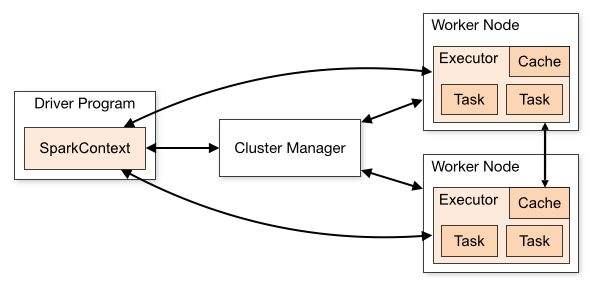
\includegraphics[width=\textwidth]{figures/spark-cluster.png}
    \caption{
      Schematics of a Spark cluster with two workers, each of them with one exectuor and two threads per executor.
      Source: Apache Spark Documentation, https://spark.apache.org/docs/latest/cluster-overview.html
    }
    \label{fig:spark-cluster}
\end{figure}

In Spark, each physical machine is called a \textit{worker}.
On each worker, Spark starts one or multiple Spark processes in their own JVM instance; each of them is called \textit{executor}.
Nowadays, many Spark deployments use a single executor per worker\footnote{This is the setup Databricks uses; Databricks is the leading
maintainer of the Spark platform and offers professional deployment to many customers.}.
Each executor runs multiple threads (often one per core on its worker) to execute multiple tasks in parallel.
In total, a Spark cluster can run \textit{\# workers} $\times$ \textit{\# executors per worker} $\times$ \textit{\# threads per executor} tasks
in parallel.

Spark uses two kinds of processes to execute an application: a \textit{driver program} and multiple \textit{executors}.
When started, the driver program acquires resources from the \textit{cluster manager} for its executor processes.
These executors stay alive during the whole Spark application.
Then, the driver program continues executing the Spark application.
When it encounters parallelizable tasks, it schedules them on the available executors.

All tasks scheduled on the same executor share a cache for in-memory data structures like \textit{Broadcast variables} or persisted RDD
partitions.
This is important in the context of this thesis because it means that we cache the input graph once per executor;
which in many Spark deployments is once per worker or physical machine.
This would not be possible if different tasks in the same JVM would not share the same cache.

Spark allows the user to choose a cluster manager to manage resources in the cluster.
It comes with good integration for Hadoop YARN~\cite{yarn}, Apache Mesos~\cite{mesos} and Kubernetes~\cite{kubernetes}, as well as,
a standalone mode where Spark provides its own cluster manager functionality.
Finally, one can run Spark on a single machine in \textit{local mode}.
In local mode, the driver program and a single executor share a single JVM.
The executor uses the cores assigned to Spark to run multiple worker threads.
For our experiments, we run Spark purely in local mode.

\subsubsection{Catalyst} \label{subsubsec:catalyst}
Catalyst~\cite{spark-sql} is Spark's query optimizer.
It can process queries given as a SQL string or described using the DataFrame API.
From a given query it constructs an executable \textit{physical plan}.
The query compilation process is organized in multiple stages.
Its inputs and stages are shown in~\cref{fig:catalyst-stages}.
Below we explain these in order.
We use the triangle given by the datalog rule $COUNT(triangle(A, B, C)) \leftarrow R(A, B), S(B, C), T(A, C), A < B < C $ as
a running example.

\begin{figure}
    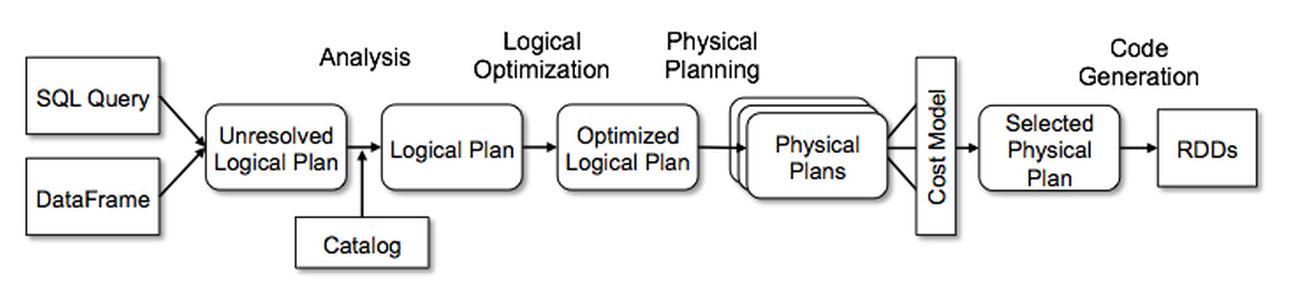
\includegraphics[width=\textwidth]{figures/catalyst-stages.png}
    \caption{
    Input and stages of the Catalyst optimizer.
    Source: Databricks Blog, https://databricks.com/blog/2015/04/13/deep-dive-into-spark-sqls-catalyst-optimizer.html
    }
    \label{fig:catalyst-stages}
\end{figure}

The input of Catalyst is a query in the form of a DataFrame or SQL string.
From this the optimizer builds a \textit{unresolved logical plan}.
This plan can include unresolved attributes, e.g. attribute names which are not matched to a specific
data source yet or which have no known type.
To resolve this attributes Catalyst uses a \textit{Catalog} of possible bindings which describe the
available data sources.
This phase is referred to as \textit{Analysis} and results in a \textit{logical plan}.
The logical plan represents \textit{what} should be done for the query but not exactly \textit{how},
e.g. it might contain a Join operator but not a Sort-merge join.

We show the logical plan for the triangle query in~\cref{fig:triangle-logical-plan}.
As we see, the query is represented as tree where the vertices are operators and the edge indicate dataflow from
one operator to another.
The leaves of the tree are three aliases of the edge relationship.
zTwo of these source relationships are the input the join between \textit{R} and \textit{S} via \textit{B}.
The result of this join and the leaf relationship \textit{T} are input to the second join.
The tuples produced by this join are filtered to fulfil $A < B < C$.
Finally, at the root of the tree, there is an aggregation to count all results and report the sum.

\begin{figure}
    \centering
    \subfloat[Logical plan\label{fig:triangle-logical-plan}]{\includesvg[width=0.4\textwidth]{triangle-logical-plan}}
    \subfloat[Physical Plan\label{fig:triangle-physical-plan}]{\includesvg[width=0.6\textwidth]{triangle-physical-plan}}
    \caption{Logical and physical plan for the triangle count query as generated by Catalyst.}
\end{figure}

The \textit{logical optimization phase} applies batches of rewriting rules until a fixpoint is reached.
A simple example of a logical optimization would be rewriting $2 + 2$ into $4$.
In the running example of the triangle query, this phase pushes the filters into the two joins.
This optimization is called Filter Pushdown.
It is efficient because it applies filters earlier within the pipeline reducing the number tuples to process by later operators.

From the \textit{optimized logical plan} the optimizer generates one or multiple \textit{physical plans} by
applying so called \textit{Strategies}.
They translate a logical operator in one or multiple \textit{physical operators}.
\textit{Strategies} are also allowed to return multiple physical plans for a single \textit{logical plan}.
In this case, the optimizer selects the best one according to a \textit{cost model}.

The physical plan for the triangle query is shown in~\cref{fig:triangle-physical-plan}.
We see multiple examples of translation of a logical operator, which describes what to do, to its physical pendant that also
describes how to do it: the \textit{TableScan} becomes a \textit{CSVRead} and the \textit{Joins} are implemented as
\textit{BroadcastHashJoins}.

Furthermore, we see the introduction of exchanges.
\textit{BroadcastExchanges} precede the \textit{BroadcastHashJoins}.
They build a hashtable from their input operators and make them available as a broadcast variable to all executors of the cluster;
we explain broadcast variables in depth in~\cref{subsubsec:broadcast-variables}.
When an executor is tasked to execute the hash join operator, it acquires the broadcasted hashtable and executes a local hash join
of its assigned partitions.

Another exchange operator is introduced for the aggregation.
It is broken up into a partial aggregation directly after the last join, an exchange reorganizing all partial counts into a single
partition and a second aggregation over that partition to calculate the total count.
The last is a good example of Catalyst introducing a shuffle.

To conclude, the translation to a physical plan translates logical operators into concrete implementations of these and adds exchanges
to organize the data such that it can be processed independently in partitions.

After generating and choosing a physical plan, Catalyst enters the \textit{code generation} phase in which it compiles Java byte code for
some of the physical operators.
This code executes often magnitudes faster than interpreted versions of the same operator~\cite{spark-sql} because
it can be specialized towards this particular query, e.g. if a join operates only on integers, code
generation can prune all code paths dealing with strings.
Indeed, the code generation phase is part of another Spark project called
\textit{Tungsten}~\cite{tungsten-project,tungsten-code-generation}.
In this thesis, we do not build any code generated physical operators.
Hence, we do not treat this topic in depth.
It is enough to know that all freshly generated Java code is wrapped into a single physical operator.
Therefore, it integrates seamlessly with interpreted operators.

Finally, Catalyst arrives at an optimized physical plan which implements the query.
The execution of this plan is called
\textit{structured query execution}~\cite{spark-internals-structured-query-execution}.
It translates the plan into RDD operations implemented by Spark's core.
Hence, the result of Catalysts query compilation is an RDD representing the query.
One should note that structured query execution does not materialize the query: the result is an RDD which is a none
materialized representation of the operations necessary to generate the result.
In this thesis, we are not concerned with the internals of RDD's.
We do not need to introduce any new RDD operations or even touch Spark's core functionality.
Thanks to the extensibility of Catalyst, we can integrate worst-case optimal joins by adding one logical operator, multiple
physical operators and a Strategy to translate between them.

\subsubsection{Broadcast variables} \label{subsubsec:broadcast-variables}
\textit{Broadcast variables} readonly variables which are accessible by all tasks.
They are initialized once by the driver program and should not be changed after initialization.
The process of broadcasting them is handled by Spark.
It is guaranteed that each broadcast variable is sent only once to each executor and allows it to be spilled to disk if it is not
possible to keep the whole value in memory.
Furthermore, `Spark attempts to distribute broadcast variables using efficient broadcast algorithms to reduce communication
costs'~\cite{rdd-programming-guide}; currently Spark uses a BitTorrent-like communication protocol\footnote{See Spark sources:
\texttt{org.apache.spark.broadcast.TorrentBroadcast}}.
Once sent, they are cached once per executor~(see also~\cref{subsubsec:spark-architecture}) and shared by all tasks on this executor.
They are cached in deserialized form in memory but can be spilled to disk if they are too big.
In this thesis, we use broadcast variables to cache the edge relationship of the graph on all workers.

\subsection{Graph pattern matching}
% Definition of graph pattern matching
% Important queries can be covered by full, conjugutive E1 formulaes
% Worst-Case Optimal Algorithms for Parallel Query Processing, contains great background on conjugutive queries
%  or equijoins
%

\subsection{Worst-case optimal join algorithm}\label{subsec:worst-case-optimal-join-algorithm}
The development of worst-case optimal joins started in 2008 with the discovery that the output size of a relational query
is bound by the fractional edge number of its underlying hypergraph~\cite{agm}.
In short, this bound proves that traditional, binary join plans perform asymtopically worse than theoretical possible
for the worst-case database instances, e.g. heavely skewed instances.
For example, the worst-case runtime of binary joins on the triangle query is in $\mathcal{O} (N^2)$, while the AGM bound
shows the possibility to solve it in $\mathcal{O} (N^{3/2})$.
The AGM bound has been treated widely in literature~\cite{skew-strikes-back,andreas,agm}.
A particular good explanation is given by Hung Ngo et al in~\cite{skew-strikes-back}.
We refer the reader to these papers for further information.
In the next paragraph, we discus different algorithms matching the AGM bound which are called worst-case optimal joins.

In 2012, Ngo, Porat, Re and Rudra published the first join algorithm matching the AGM bound, called \textit{NPRR} join~\cite{nprr}.
In the same year, Veldhuizen proved that the algorithm Leapfrog Triejoin used in LogicBlox,
a database system developed by his company, is also worst-case optimal with regards to the fractional edge number bound.
We often abbreviate Leapfrog Triejoin to \textsc{LFJT}.
Both algorithms have been shown to be instances of a single algorithm, the \textit{Generic Join}, in 2013 by Ngo et al.~\cite{skew-strikes-back}.

Three worst-case optimal join algorithms are known in literature.
We choose Leapfrog Triejoin as the basis for our work.
The argumentation for this decision is given below.
First, we identify the main criteria for this choice.
Then, we use them to compare the different algorithms.

The most important argument for our decision is the degree to which the algorithm has been shown
to be of practical use.
In particular, the number of systems it is used in and openly available data on its performance.
If an algorithm is used in academia as well as in industry, we deem this as a advantage.
This criteria carries a lot of weight because the first literature on worst-case optimal joins
has been rather theoretical but in our work we take a more praxis and system oriented perspective.

The practical character of our work also motivates the second dimension which we compare the algorithms in, namely
ease of implemenation.
If two of the three algoritms both have well proven performance, we would like to choose the algorithm
that takes less time to implement and is easier to adapt and experiment with.
That is, to be able to spent more time on evaluation and optimizations for the graph use-case, instead of,
time spent on replicating existing work.

The Leapfrog Triejoin is used in two commercial database solutions:
LogicBlox~\cite{logicBlox} and RelationalAI\footnote{https://www.relational.ai/}.
Its performance has been reported on in two publications~\cite{myria-detailed,olddog}.
In particular, it beats various general and graph specific databases for graph pattern matching, i.e.
PostgresSQL, MonetDB, NEO4J, graphLab and Virtuoso~\cite{olddog}.
The broadest study of its performance uses 15 different datasets and 7 queries~\cite{olddog}.
We conclude that the performance of \textsc{LFTJ} is well established by peer reviewed publications
as well as industrial usage.

The \textit{NPRR} algorithm has been well analyzed from the theoretical point of view.
However, we are not able to find any openenly available sources with performance measurements.
This disqualifies \textsc{NPRR} as basis for our thesis.

The \textit{Generic Join} is used in at least three academic graph processing engines,
namely GraphFlow~\cite{graphflow}, EmptyHeaded~\cite{emptyheaded} and a unnamed implementation in
Timely Dataflow~\cite{ammar2018distributed}.
All three show good performance.
However, we are not aware of any commercial systems using \textsc{GJ}.

The comparision of Leapfrog Triejoin, \textsc{NPRR} and \textit{Generic Join} by proven performance
rules out \textsc{NPRR} and puts \textsc{LFTJ} and \textsc{GJ} on a similar level.
Next, we compare these two algorithm in ease of implementation.

The description of the Leapfrog Triejoin implementation in its original paper~\cite{lftj} is excellent.
Furthermore, multiple open source implementation exists~\cite{leapfrog-triejoin-schroeder,myria-detailed}.
In particular, the implementation of Christian Schroeder for a course at Oxford is helpful because it is standalone and
does not require us to understand a whole system\footnote{https://github.com/schroederdewitt/leapfrog-triejoin}.

\textit{Generic Join} is described as a generalization of \textsc{NPRR} and Leapfrog Triejoin in its original
paper~\cite{skew-strikes-back}.
Although, well written and algorithmically clear, this explanation is much less practical than the one given for \textsc{LFTJ} which
is backed by an executable implementation.

To conclude, we choose Leapfrog Triejoin as basis for our work based on its openely available records of performance, use in
academia as well as industrial systems and good description for direct implementation.
Furthermore, Peter Boncz (supervisor of this thesis) has direct contact to the inventors of \textsc{LFTJ} giving us access to valuable
expertise if necessary.

\subsubsection{Leapfrog Triejoin} \label{subsubsec:leapfrog-triejoin}
In this section, we described the Leapfrog Triejoin algorithm.
In the first paragraph, we give the high-level idea behind the algorithm and some of its requirements.
Then we discuss the kind of queries that can be answered with it.
The main part of the section, discusses the conceptual algorithm itself.
We finish with a short discussion of two implementation problems, namely the data structure to represent the input relationships and
the problem of choosing a good variable ordering.

The Leapfrog Triejoin is a variable-oriented join.
Given an input queries, it requires a variable ordering.
For example in the triangle query $triangles(a, b, c) \leftarrow R(a, b), S(b, c), T(a, c)$,
the variable ordering could be $a, b, c$.
Furthermore, the Leapfrog Triejoin requires its input relationships to be sorted by lexicographic, ascending order over the given
variable ordering, e.g. $R$ needs to be sorted by primarily by $a$ and secondary by $b$ given the variable ordering $a, b, c$.
The algorithm is variable-oriented because it fixes one possible binding for $a$, one for $b$ given $a$ and finally one for $c$ given $a$
and $b$.
This allows it to enumerate the result of the join query without intermediary results.
The process can be thought of as a backtracking, depth-first search for possible bindings.

The algorithms impelemted in this thesis can process joins of the full conjunctive fragment of first order logic or conjunctive
equi-joins in relational algebra terms.
Possible extentsions to disjunctions, ranges (none-equi joins), negation, projection, functions and scalar operations on join variables are
explained in the original Leapfrog Triejoin paper~\cite{lftj}.
However, they are not relevant to the core of this work because many interesting graph patterns can be answered using the full conjunctive
fragment, e.g. cliques or cycles.

The Leapfrog Triejoin algorithm uses three components which are composed in a layered fashion.
The concrete composition used for the triangle query is shown in~\cref{fig:lftj-layers}.
In this figure, we see three layers each of them made of one or more instances of a component.
The components are the \textit{TrieIterator}, \textit{LeapfrogJoin} and \textit{LeapfrogTriejoin}.
In the next paragraphs, we explain each layer in order, starting with the lowest layer.

\begin{figure}
    \includesvg[width=\textwidth]{lftj-layers}
    \caption{
    The three layers of the Leapfrog Triejoin algorithm.
    The configuration for a triangle query is shown: three \textit{TrieIterators} one
    per input relationship, three \textit{LeapfrogJoins} one per variable and
    one \textit{LeapfrogTriejoin} component are neccessary.
    The arrows indicate that a component uses another.
    The \textit{LeapfrogTriejoin} uses all other components but only the vertical part of the \textit{TrieIterators} (dashed arrows).
    The \textit{LeapfrogJoins} uses the linear part of two \textit{TrieIterators} each.
    }
    \label{fig:lftj-layers}
\end{figure}

The lowest layer is made of one \textit{TrieIterator} per input relationship.
In our example, we have three instances one for R, S and T each.
The \textit{TrieIterator} interface represents the input relationship as a trie with all values for
the first attribute on the first level, the values for the second attribute on the second level and so
on; an example for this is shown in~\cref{fig:trie-example}.

\begin{figure}
    \centering
    \includesvg[height=5cm]{trie}
    \caption{A 3-ary relationship as table (left) and trie (right), to position the iterator at the tuple (1, 1, 5) one
    calls \textit{open} twice, \textit{key} returns now 5, after a call to \textit{next}, \textit{key} returns 6 and \textit{up}
    would lead to \textit{key} returning 1.}
    \label{fig:trie-example}
\end{figure}

The trie contains one level per attribute of the relationship;
in the case of the triangle query, there are two levels: one for $a$ and one for $b$.
Each level is made of all possible values for its attribute.
All tuples of the relationship can be enumerated by a depth-first traversal of the trie.

The \textit{TrieIterator} component offers six methods shown in~\cref{table:trieIterator-interface}.
The \textit{open} and \textit{up} methods control the level the iterator is positioned at;
\textit{open} moves it one level down and \textit{up} moves it one level up.
Additionally, \textit{open} places the iterator at the first value for the next level and the up
method returns to the value of the upper level that was current when the deeper level was opened.
We call these two methods the vertical component of the \textit{TrieIterator} interface.

\begin{table}
    \centering
    \begin{tabular}{@{}ll@{}}
        \toprule
        Method         & required complexity    \\
        \midrule
        int key()      &  $\mathcal{O}(1)$       \\
        bool atEnd()   &  $\mathcal{O}(1)$       \\
        void up()      &  $\mathcal{O}(\log_N)$  \\
        void open()    &  $\mathcal{O}(\log_N)$  \\
        void next()    &  $\mathcal{O}(\log_N)$  \\
        void seek(key) &  $\mathcal{O}(\log_N)$  \\
        \bottomrule
    \end{tabular}
    \caption{
      The \textit{TrieIterator} interface with required complexity.
      $N$ is the size of relationship represented by the iterator.
    }
    \label{table:trieIterator-interface}
\end{table}

The other four methods are called linear component.
All of them operate on the current level of the \textit{TrieIterator}.
The \textit{key} function returns the current key (a single integer).
The \textit{next} method moves the iterator to the next key on the same level.
The \textit{seek(key)} operation finds the least upper bound for its parameter \textit{key}.
Finally, the \textit{atEnd} method returns \textit{true} when the iterator is placed behind the last value of the current level.

The middle layer of the Leapfrog Triejoin is made of one \textit{LeapfrogJoin} per variable in the join.
This join generates possible bindings for its variable by intersecting the possible values for all input relationship containing the
variable.
Therefore, it operates on the linear component of all \textit{TrieIterators} of relationships with this variable.
\Cref{fig:lftj-layers} for the triangle query shows three \textit{LeapfrogJoin} instances (for $a, b$ and $c$);
each of them uses two \textit{TrieIterators}.

The \textit{LeapfrogJoin} interface has five methods shown in~\cref{table:leapfrogJoin-interface}, with their required asymptopical
performance.
In the following paragraphs, we explain each of them.
In short, the join offers an iterator interface over the intersection of its input iterators.
This intersection is found by repeatingly seeking the value of the largest input iterator in the smallest input iterator.
This process resemples a frog taking a leap which gives the join its name.
When all iterators point to the same value leapfrogging stops and the value is emitted as part of the intersection.

\begin{table}
    \centering
    \begin{tabular}{@{}ll@{}}
        \toprule
        Method         &  required complexity    \\
        \midrule
        int key()      &  $\mathcal{O}(1)$       \\
        bool atEnd()   &  $\mathcal{O}(1)$       \\
        void init()    &  $\mathcal{O}(\log_N)$  \\
        void next()    &  $\mathcal{O}(\log_N)$  \\
        void seek(key) &  $\mathcal{O}(\log_N)$  \\
        \bottomrule
    \end{tabular}
    \caption{
    The \textit{LeapfrogJoin} interface with required complexity.
    $N$ is the size of relationship represented by the iterator.
    }
    \label{table:leapfrogJoin-interface}
\end{table}


The \textit{init} operation sorts the input iterator by their current key and finds the first value of the intersection.
To find the first value it uses the private method \textit{leapfrogSearch} which is the work-horse of the whole join.
The algorithm of this method is shown in~\cref{alg:leapfrogSearch}.
This method loops the process of calling the \textit{seek} method of the its smallest input iterator with the key of the largest input
iterator until the smallest and the largest (and therefore all iterators) point to the same value.


\begin{algorithm}
    \KwData{\\
      iters \textit{sorted array of TrieIterators} \\
      p \textit{index of the smallest iterator}
    }
   \KwResult{\textit{Either} atEnd \textit{is true or} key \textit{is set to next key of intersection}}
    maxKey $\gets$ iters[p \% iters.length].key()\;
   \While{\upshape iters[p].key() $\neq$ maxKey}{
     iters[p].seek(maxKey)\;
     \eIf{\upshape iters[p].atEnd()} {
       atEnd $\leftarrow$ true\;
       \Return\;
     } {
       maxKey $\leftarrow$ iters[p].key()\;
       p $\leftarrow$ (p + 1) \% iters.length\;
     }
   }
   key $\leftarrow$ iters[p].key()
   \caption{leapfrogSearch()}
   \label{alg:leapfrogSearch}
\end{algorithm}
% TODO styling


The \textit{leapfrogNext} method moves the join to its next value.
Internally, it uses the \textit{next} function of its smallest iterator and then \textit{leapfrogSearch}.

The operation \textit{leapFrogSeek(key)} first uses the \textit{seek} method of the smallest input iterator to forward it to \textit{key};
then it uses \textit{leapfrogSearch} to either verify that this key is available in all iterators (hence in the intersection) or
to find the upper bound of this key.

Finally, the functions \textit{key} and \textit{atEnd} return the current key or if the intersection is complete respectively.

% TODO line numbers
The last layer of the whole algorithm is a single \textit{LeapfrogTriejoin} instance.
It interacts with both lower layers to enumerate all possible bindings for the join.
For this it aquires one binding for the first variable from the corresponding \textit{LeapfrogJoin}.
Then it moves the \textit{TrieIterators} containing this variable to the next level and
finds a binding for the second variable using the next \textit{LeapfrogJoin}.
This process continues until all variables are bound and a tuple representing this binding is emitted
by the join operator.
Then it finds the next possible binding by backtracking.

\Cref{alg:leapfrogTrieJoin-state-machine} shows the backtracking depth-first traversal.
This traversal needs to stop each time when a complete tuple has been found to support the iterator interface of the join.
Therefore, it is implemented as a state-machine which stops each time the deepest level is reached and all variables are bound
(loop condition in line 33). % LINE
The next action of the state machine is determined by the outcome of the current action.
Hence, we can characterize the state machine by describing each possible action and its possible outcomes.
There are three possible actions: \textit{next}, \textit{down} and \textit{up}.
We summarize the possible actions, conditions for the next action and if the main loop of the state machine yields the next tuple
in~\cref{table:lftj-state-machine} and describe each action below.

\begin{algorithm}
    \KwData{
      depth \textit{the index of the variable to find a binding for, ranges from -1 to \#variables - 1}\\
      bindings \textit{array holding the current variable bindings or $-1$ for no binding} \\
      MAX\_DEPTH \textit{the number of variables - 1} \\
      action \textit{state of the state machine}
    }
    \Repeat{\upshape $\neg$ (depth = MAX\_DEPTH $\and$ bindings[MAX\_DEPTH] $\neq$ -1) $\lor$ atEnd} {
      \Switch{\upshape action} {
        \Case{\upshape NEXT} {
            leapfrogJoins[depth].leapfrogNext() \; \label{line:lftj-leapfrog-next}
            \eIf{\upshape leapfrogJoins[depth].atEnd()} {
                action $\leftarrow$ UP \; \label{line:lftj-next-up}
            } {
                bindings(depth) $\leftarrow$ leapfrogJoins[depth].key() \; \label{line:lftj-next-down-or-next}
                \If{\upshape depth == MAX\_DEPTH} {
                    action $\leftarrow$ NEXT
                } {
                    action $\leftarrow$ DOWN
                }
            }
        }
       \Case{\upshape DOWN} {
          depth $\leftarrow$ depth + 1 \;
          trieJoinOpen() \; \label{line:lftj-trieJoinOpen}
          \eIf{\upshape leapfrogJoins[depth].atEnd()} {
            action $\leftarrow$ UP \; \label{line:lftj-down-up}
          } {
            bindings(depth) $\leftarrow$ leapfrogJoins[depth].key() \;
          \eIf{\upshape depth = MAX\_DEPTH} {
             action $\leftarrow$ NEXT \label{line:lftj-down-next}
          } {
            action $\leftarrow$ DOWN
          }
          }
       }
        \Case{\upshape UP} {
          \eIf{\upshape depth = 0} { \label{line:lftj-atEnd}
            atEnd $\leftarrow$ true \;
          } {
            depth $\leftarrow$ depth - 1 \;
            trieJoinUp() \; \label{line:lftj-trieJoinUp}
            \eIf{\upshape leapfrogJoins[depth].atEnd()} { \label{line:lftj-up-up-next}
                action $\leftarrow$ UP \;
            } {
                action $\leftarrow$ NEXT \;
            }    
          }
        }
      }
    }  
    \caption{LeapfrogTrieJoin state machine}
    \label{alg:leapfrogTrieJoin-state-machine}
    % TODO mention triejoinopen and triejoinUP
\end{algorithm}

The \textit{next} action moves the \textit{LeapfrogJoin} at the current depth to the next possible binding for its variable
(line~\ref{line:lftj-leapfrog-next}).
If the \textit{LeapfrogJoin} reached its end, we continue with the \textit{up} action (line~\ref{line:lftj-next-up}),
otherwise we set the binding and continue by another \textit{next} action, if we are at the deepest level or by moving
to the next deeper level by the \textit{down} action (line~\ref{line:lftj-next-down-or-next}ff).

The \textit{down} action moves to the next variable in the global variable ordering by opening all related \textit{TrieIterators}
and initializing the corresponding \textit{LeapfrogJoin} (line~\ref{line:lftj-trieJoinOpen} call to \textit{trieJoinOpen}).
A \textit{down} can be followed by an \textit{up} if the \textit{LeapfrogJoin} is \textit{atEnd} (line~\ref{line:lftj-down-up}),
by a \textit{next} action if the trie join is at its lowest level (line~\ref{line:lftj-down-next}), or by another \textit{down} action to
reach the deepest level.

The \textit{up} action can signal the completion of the join if all bindings for the first variable in the global ordering have
been explored, or in other words, the first \textit{LeapfrogJoin} is \textit{atEnd} (condition
\textit{depth == 0 $\wedge$ action ==  UP} line~\ref{line:lftj-atEnd}).
Otherwise, all \textit{TrieIterators} corresponding to the current variable are moved upwards by calling \textit{triejoinUp}
(line~\ref{line:lftj-trieJoinUp}) which also updates \textit{depth} and \textit{bindings}.
Then, this action is followed by another \textit{up} or a \textit{next} depending on \textit{atEnd} of the current \textit{LeapfrogJoin}
(lines~\ref{line:lftj-up-up-next}).

\begin{table}[]
    \centering
    \begin{tabular}{@{}llll@{}}
        \toprule
        Action                & Condition                                  & Next action & Yields \\ \midrule
        \multirow{3}{*}{NEXT} & \textit{lf.atEnd}                                   & UP          & no     \\
        & \textit{$\neg$lf.atEnd} $\wedge$ \textit{reachedMaxDepth}             & NEXT        & yes    \\
        & \textit{$\neg$lf.atEnd} $\wedge$ \textit{$\neg$reachedMaxDepth}            & DOWN        & no     \\
        & & &\\
        \multirow{3}{*}{DOWN} & \textit{lf.atEnd}                                   & UP          & no     \\
        & \textit{$\neg$lf.atEnd} $\wedge$ \textit{reachedMaxDepth}             & NEXT        & yes    \\
        & \textit{$\neg$lf.atEnd} $\wedge$ \textit{$\neg$reachedMaxDepth}            & DOWN        & no     \\
        & & &\\
        \multirow{3}{*}{UP}     & \textit{depth = 0}, means highest \textit{lf.atEnd} is true & -- (done)         & yes    \\
        & \textit{lf.atEnd}                                   & UP          & no     \\
        & \textit{$\neg$lf.atEnd}                                  & NEXT        & no     \\ \bottomrule
    \end{tabular}
    \caption{Summary of actions, conditions for the following action and if a complete tuple has been found.
    \textit{reachedMaxDepth} is true if we currently find bindings for the last variable in the global order.
    \textit{lf} abbreviates the \textit{LeapfrogJoin} of the current variable.
    The columns \textit{Yields} details if the main loop of the state machine yields before computing the next action,
    this is the case, when all variables have been bound.
    }
    \label{table:lftj-state-machine}
\end{table}

% TODO positioning
\paragraph{TrieIterator implementation, backing data structure}
While we can implement the \textit{LeapfrogJoin} and \textit{LeapfrogTriejoin} component of the Leapfrog Triejoin from the
algorithmic description given above, we are missing some details for a concrete implementation of the
\textit{TrieIterator} interface.
Mainly, we need to decide for a datastructure to back the \textit{TrieIterator}.

We choose to use sorted arrays as described in~\cite{myria-detailed}.
One array is used per column of the input relationship and binary search on these arrays allows us to implement the \textit{TrieIterator}
interface with the required asymptopical complexities (see~\cref{table:trieIterator-interface}).

%We briefly compare a B-tree v.s. array-based implementation of
%the LFTJ API. The main API function is seek(v), which fetches the next value v’ of the current attribute Ai s.t. v’ > v: in a B-tree this can be computed in amortized time O(1), while our implementation uses a binary search on the remaining part of the array at a cost per operation of O(log n). Thus, TJ is at most a factor log n slower than LFTJ, and, in particular, it is also worst case optimal (up to log n). In practice, the dominating cost of TJ is given by the sorting phase (which, as explained, is unavoidable), hence our choice to use a sorted array instead of a B-tree, because sorting is cheaper than computing a B-tree.

\paragraph{Variable ordering}  % TODO move all sections one up and use of chapter?
Finding a good variable ordering for the \textsc{LFTJ} is an interesting research problem in itself.
We are aware of two existing approaches.

The first is to create and maintain representative samples for each input relationship and determine the best order based on runs over
these samples.
This has been implemented in LogicBlox, the first system to use Leapfrog Triejoins~\cite{logicBlox}.
To the best of our knowledge, the exact method of creating the representative samples has not been published.

The second approach is described in great detail by Mhedhbi and Salihoglu in~\cite{mhedhbi2019}.
Its has been implemented in their research graph database Graphflow~\cite{graphflow}.

They define a novel cost-metric for \textsc{WCOJ}s which estimates the costs incured by constructing the intersections of adjacency
lists.
The metric takes three factors into account.
First, the size adjacency lists.

% TODO tailed triangle query, all other query pics for experiments
Second, the number of intermediate matches.
The concept of intermedieate matches is best understood by a simple example;
we see the tailed-triangle query in~\cref{fig:tailed-triangle}.
Two very different vertice ordering categories exist for this query.
The ones that start on $v_4$ and find all 2-paths of the graph;
and vertice orderings that start with $v_1, v_2, v_3$ in any order which close the triangle first.
Clearly, there are more 2-paths in any graph than triangles.
Hence, the second category produces far less intermediate matches.

Finally, they implement an intersection cache in their system which takes advantage of the fact that some queries can reuse already
constructed intersections.
So, the last factor taken into account by their cost metrics is the usage of this intersection cache.

They use the described cost metric, a dynamic programming approach to enumerate possible plans and  a catalogue of sampled subgraph
instances containing the sizes of adjacency lists to intersect and produced intermediate results to estimate the costs for all
variable orderings.

Moreover, they implement the ability to change the query ordering adaptively during query execution  based on the real adjacency list sizes
and intermediate results.
They show that adaptive planning can improve the performance of many plans.
Furthermore, it makes the query optimizer more robust against choosing bad orderings.

To conclude, the work of Mhedhbi et al. is the most comprehensive study on query vertex orderings for \textsc{WCOJs} currently available;
they introduce a cost metric, a query optimizer to use this metric and prove that it is possible and beneficial to compute parts of
the results using a different variable order.

In our work, we do not implement an automatic process to choose the best variable order.
The order we choose is based on experiments with different orders and intuition of the author.

Integrating the approach of LogixBlox would be possible but require the implementer to find a good sampling strategy because no details
are openenly available.

The approach of Mhedhbi and Salihoglu is much better documented but also more complex.
It consists out of four contribution which build up on each other but could be useful on its own.
The cost metric described in their paper applies to our system as well and could be used.

They use this metric for cost estimation in connection with a none-trivial subgraph catalogue.
The main challenge in integrating this way of cost estimation with our system is to elegantly integrate catalogue creation in Spark.

Their solution for adaptive variable orderings is helpful because it proves that this technique is beneficial;
they also publish performance measurements, so the impact can be evaluated.
However, there system employs a \textit{Generic Join} while we use a Leapfrog Triejoin.
The integration of adaptive variable orderings into Leapfrog Triejoin is not trivial and it is likely that their implementation is not
directly applicable.

Finally, they introduce an intersection cache to make use of repeatedly used intersections.
This can be directly applied to our system, e.g. using the decorator pattern around \textit{LeapfrogJoins}.
We note that they only cache the last, full n-way-interesection of multiple adjacency lists.
It would be interesting to research if the system would benefit from caching partial n-way intersections as well because
we noticed that for some queries, e.g. 5-clique, the intersection between the first two lists can be reused more often than the full
intersection.
This opens the interesting question in which order we should intersect the lists.

We conclude that two concepts to choose a good variable ordering exists which are both (partially) applicable to our system.
The LogixBlox approach is simpler and directly integratable but not well documented.
The solution used in GraphFlow is far more complex and developed for another \textsc{WCOJ}.
Anyhow, the paper describes it in great detail and parts of it could be integrated directly, while others need some engineering effort or
need to be redesigned completely.


% Additional ideas.
%===================
% Queries: olddog, Semih's paper,
%    Mostly for graphs

% background over "typical" graph pattern matching queries needed
%   olddog good introduction about binary joins vs wcoj for graph pattern matching
% background about graph pattern matching needed


% WCOJ against graph engines (oldog)
% Comparision with other systems: oldog, graphlab, virtuoso, monetdb, pssql, neo4j

% comparision, intermediate results
%  intuitive understanding of why better?
% background on binary join operators?

% Codegeneration studied by RelationalAi
% Compression studied by Richard

% OLD
%====
%We implement the Leapfrog Triejoin~\cite{leapfrog} as our general sequential version of a WCOJ.
%However, instead of using B-Trees as a backing data structure, we use sorted arrays and a binary
%search, which has been described in~\cite{myria-detailed} and is called
%Tributary join in their paper.
%Our Leapfrog Triejoin is implemented in three components which we explain in order below: \textit{LeapfrogJoin}, \textit{ArrayTrieIterable} and
%\textit{LeapfrogTriejoin}.
%
%The Leapfrog join is a variant of the sort-merge join for unary relationships, originally described in~\cite{leapfrog1,leapfrog2}. % TODO see LFTJ paper 4 and 7
%To join $k$ unary relations $A_1(x)$, $A_2(x)$, \dots, $A_k(x)$ it takes one iterator per input relations and offers an iterator
%interface that yields the intersection of all relations.
%It requires that it's input iterators offer a \textit{key} method in $\mathcal{O}(1)$, a \textit{next} method and
%a \textit{leastUpperBound(key: Int)} both in $\mathcal{O} (\log n)$ ($n$ defined as the size of the input relationship).
%\textit{leastUpperBound} moves the iterator to the first position of the sought \textit{key} or the first position of the
%next higher value.
%An idiotmatic implementation of a Leapfrog join is shown in~\cref{lst:leapfrog-join}, for the optimized implementation see
%\texttt{leapfrogTriejoin.LeapfrogJoin} in our repository.  % CODEREF

%\begin{listing}[H]
%    \inputminted[linenos=true]{scala}{code/LeapfrogJoin.scala}
%    \caption{Leapfrog join.}
%    \label{lst:leapfrog-join}
%\end{listing}

%To support j-arity relations, $A(a_1, a_2, \dots, a_j)$ we add two methods to the iterator interface that represents the input
%relationships: \textit{up} and \textit{open}; both are required to work in $\mathcal{O} (\log n)$.
%We call this new iterator Trieiterator because it represents the relationship as a trie, see~\cref{fig:trie-example}.

%The implementation of a Trieiterator backed by a columnwise representation of the relation using one array
%per column is straight forward, we outline the basic ideas here and refer the interested reader to
%\texttt{leapfrogTriejoin.ArrayTrieIterable.TrieIteratorImpl} in our repository for further details.  % CODEREF
%It helps to think about the Trieiterator as consisting out of a linear component, containing the functions
%\textit{key}, \textit{next} and \textit{leastUpperBound}, and horizontal component, made off the functions \textit{up} and \textit{open},
%to move the linear component from one trie level to another.
%
%First, we explain the horizontal component.
%They keep track of the current \textit{level} of the Trieiterator and the \textit{startPosition} and \textit{endPosition}
%for in the column, e.g. in~\cref{fig:trie-example} when the current \textit{level} is 1 (or x), the key equals 4, the
%\textit{startPosition} is 2 and
%the \textit{endPosition} is 5 because the value 4 occurs 3 times.
%With these bookkeeping variables, updated by \textit{up} and \textit{open}, one can implement the linear part by
%a binary search over the current column (given by \textit{level}) which is limited to \textit{startPosition} and \textit{endPosition}.
%
%\begin{figure}
%    \centering
%    \includesvg[height=5cm]{trie}
%    \caption{A 3-ary relationship as table (left) and trie (right), to position the iterator at the tuple (1, 1, 5) one
%    calls \textit{open} twice, \textit{key} returns now 5, after a call to \textit{next}, \textit{key} returns 6 and \textit{up}
%    would lead to \textit{key} returning 1.}
%    \label{fig:trie-example}
%\end{figure}

%The Leapfrog Triejoin combines TrieIterators and Leapfrog joins to join $k$ relationships of arbitrary arity.
%Its input is one Trieiterator per relationship, with these it builds one Leapfrog join per attribute which
%receives references to all Trieiterator of relationships containing the attribute, e.g. for the triangle query
%\textit{R(a, b), S(b, c), T(a, c)} the Leapfrog Triejoin receives three Trieiterator, for \textit{R}, \textit{S} and
%\textit{T},
%and builds three Leapfrog joins, for $a$, $b$, $c$, which receive references to two Trieiterators each.
%To generate the join result the Leapfrog Triejoin operates the horizontal components of the Trieiterators directly and
%uses the Leapfrog joins to operate the linear component.

%We show an idiomatic implementation of a Leapfrog Triejoin in~\cref{lst:leapfrog-triejoin} and~\ref{lst:leapfrog-triejoin-helpers}, a
%performance oriented
%implementation can be found in our repository in \texttt{leapfrogTriejoin.LeapfrogTriejoin}.
%These listings contain two important functions: the initialization function from line~\ref{line:lftjInitStart} to
%line~\ref{line:lftjInitEnd} % LINE
%and the \textit{moveToNextTuple} function at line~\ref{line:moveToNextTuple}. % LINE
%We go through these functions in order.

%The initializer gets two arguments: a mapping from variables to \textit{TrieIterators} (each \textit{TrieIterator} belongs to
%the list of attributes of its relationship) and the global variable ordering as a sequence of \textit{Strings}.
%First, it creates one \textit{LeapfrogJoin} per variable (line 5) which receives references % LINE
%to each \textit{TrieIterator} operating on a relationship with this attribute.
%Then it builds a mapping from variables to all \textit{TrieIterators} acting on a relationship with an attribute of the same name (line
%8). % LINE
%Finally, it initializes \textit{maxDepth}, \textit{action}, \textit{depth}, \textit{bindings} and \textit{atEnd} (line 10 to line 14). %
%LINES
%\textit{depth} and \textit{bindings} are an internal variable storing the index of the variable to bind currently and the
%current bindings for all variables up to \textit{depth}.
%\textit{atEnd} signals that the join has been completed to the client.



%\begin{listing}[H]
%    \inputminted[mathescape, linenos=true]{scala}{code/LeapfrogTriejoinIdiomatic.scala}
%    \caption{Shows the main methods of \textit{LeapfrogTriejoin}, the initializer and \textit{moveToNextTuple} functionality
%    helper methods are detailed in~\cref{lst:leapfrog-triejoin-helpers}.}
%    \label{lst:leapfrog-triejoin}
%\end{listing}
%
%\begin{listing}[H]
%    \inputminted[linenos=true]{scala}{code/LeapfrogTriejoinHelpers.scala}
%    \caption{\textit{LeapfrogTriejoin} helpers.}
%    \label{lst:leapfrog-triejoin-helpers}
%\end{listing}


\subsection{Distributed worst-case optimal join in Myria} \label{subsec:myria}
In 2014, a Leapfrog Triejoin variant, dubbed Tributary Join, was used as a distributed join algorithm on a shared-nothing architecture called Myria~\cite{myria-detailed}.
They use Tributary Join as a local, serial worst-case optimal join algorithm, combined with the Hypercube shuffle algorithm, also called
\textit{Shares}, to partition the data between their machines~\cite{shares}.
The combination of a shuffle algorithm with a \textsc{WCOJ} allows them to distribute an unchanged serial worst-case optimal join
version by running it only on a subset of the data on each worker.

This approach is directly applicable to Spark.
We could implement a hypercube shuffle for Spark and then choose any \textsc{WCOJ} to run on each partition.
However, it is not obvious how well this approach scales because Shares replicates many of its input tuples~\cite{myria-detailed}.
The experiments on Myria indicate that the combination of Hypercube shuffles and Tributary Join does not scale well.
They report a speedup of 8 on 64 workers compared to the time it takes on 2 nodes, which, although unlikely to be optimal, is not
investigated in great detail.

Therefore, we decide to analyse the expected scaling behaviour of Shares for graph pattern matching.
Our main concern is that the number of duplicated tuples in the system increases with the query size (number of vertices) and
with the number of workers added to the system.
We provide a theoretical analysis of the number of duplicated tuples for different query sizes and available workers in a later section
of this thesis (\ref{sec:shares-proof}).
As result of this investigation, we decide to not physically partition our data but to duplicate it to all workers and seek for alternative
strategy to parallelize a worst-case optimal join.

To conclude, the implementation in Myria and in particular the Shares algorithm is the starting point of this thesis.
We see it as our baseline for a distributed \textsc{WCOJ} implementation.
In the coming section, we explain Shares in detail.

We note that a implementation of a distributed worst-case optimal join on Timely Dataflow exists.
However, it is not applicable to Spark.
Therefore, we treat it in the related work section (\ref{subsec:wcoj-timely-data-flow}) of this thesis.

\subsubsection{Shares}
Shares partitions the input relationships for a multi-way join over worker nodes, such that, all tuples, which could be joined,
end up on the same worker in a single shuffle round.
Hence, it allows running any multi-way join algorithm locally after one shuffle round.
The output of the join is the union of all local results.

The idea is to organize all workers in a logical hypercube, such that each worker can be addressed by it hypercube coordinate.
Then it is straightforward to find a mapping from the attribute values of a tuple to these coordinates, so that joinable tuples
arrive on the same worker after one shuffle.

We first explain how to organize the workers in a hypercube and then how to map tuples to these workers.
Next, we treat the problem of choosing a good hypercube configuration.
Followed, by a summary about optimality of Shares.
Finally, we provide analysis of the scaling of Shares for graph pattern matching.

A hypercube is characterized by the number of dimensions and the size of each dimension.
\Cref{fig:hypercube} shows a hypercube with three dimesions labelled $a, b$ and $c$.
They have the size of 3, 2 and 2 for $a, b$ and $c$ respectively.
It is a possible configuration for the triangle query $triangle(a, b, c) \leftarrow R(a, b), S(b, c), T(a, c)$ with
12 workers.

\begin{figure}
    \centering
    \subfloat{\includegraphics[width=0.4\textwidth,valign=c]{figures/hypercube-example-table.png}}
    \hspace{0.04\textwidth}
    \subfloat{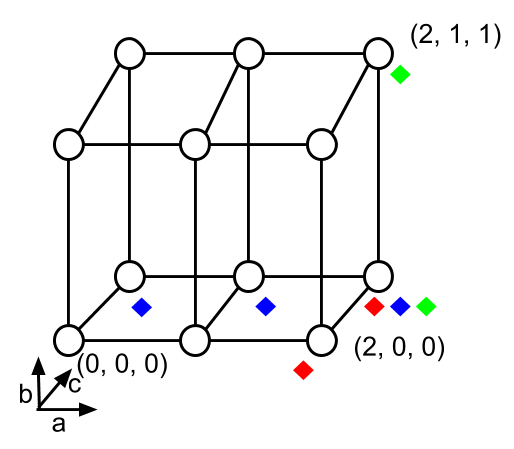
\includegraphics[width=0.55\textwidth,valign=c]{figures/hypercube-example.png}}
    \caption{
      Left: Three aliases of an edge relationship with one triangle.
        The participating tuples are marked in red, green and blue.
        Their hypercube coordinates are shown below.
      Right: Example of a Shares hypercube configuration for the triangle query for 12 workers with three attributes/dimensions of the sizes
        3, 2, 2.
        The tuples marked in red, green and blue end up on the workers with red, green and blue rhombs respectively.
    }
    \label{fig:hypercube}
\end{figure}

Given an input query, Shares builds a hypercube with one dimension per variable in the input.
It then chooses the size of each dimension, such that the product is smaller than number of workers.
We call $v$ the numbers of variables in the query and $p_0, \dots, p_v$ the sizes of each dimension.
This allows us to address each worker with a coordinate of the form $(0..p_0, \dots, 0..p_v)$.
If the product of all dimension sizes is smaller than the number of workers, additional workers are not used.
The process of finding the best sizes for the dimensions depends on the input query and the input relationships.
We discuss it in a later paragraph of this section.

With this topology in mind, it is straightforward to find a partitioning for all tuples from all relationships such that tuples that
could join are sent to the same worker.
We choose a hash function for each join variable $a$ which maps its values in the range of $[0..p_a]$.
Then each worker determines where to send the tuples it holds by hashing its values.
This results in a coordinate in the hypercube which is fixed for all join variables, which occur in the tuple, and unbounded for join
variables which do not occur in the tuple.
Then the tuple is sent to all workers with a matching coordinate.

\Cref{fig:hypercube} shows how tuples forming a triangle from three relationships are mapped to the workers.
The blue, green and red tuple in the relationships form a triangle.
The green and the red tuple are sent to 2 workers each and the blue tuple to three workers (marked with small rhombs).
They are sent to all workers along the axis where the coordinate is not determined by a value in the tuple.
We see that they all end up together on the worker with the coordinate (2, 0, 0).
This is where the triangle occurs in the output of the join.

\paragraph{Finding the best hypercube configuration}
The problem of finding the best hypercube configuration is to choose the sizes of its dimensions such that (1) the product of
all sizes is smaller than the number of available workers and (2) such that the number of tuples to single worker is minimized.
(2) is backed by the assumption that the number of tuples is a good indicator for the amount of work;
this assumption is made in all papers discussing the problem~\cite{myria-detailed,shares-proof,shares}.
Therefore, we want to minimize the number of tuples on each single worker because the slowest worker determines the run-time.
Next, we discuss existing solutions and decide for one of them.

The original Shares paper proposes a none-convex solution which is hard to compute in praxis~\cite{shares}.
Later, Beame et al. define a linear optimization problem which is solvable but leads to fractional hypercube
sizes~\cite{shares-proof}.
Hence, it is not possible to use their solution directly.
Rounding down would be an obvious solutions but as discussed in~\cite{myria-detailed}, it can lead to highly suboptimal solutions, in
particular with low numbers of workers.
Hence, the paper further considers to use a higher number of \textit{virtual} workers and assign these to \textit{physical} workers
by a one-to-many mapping.
Anyhow, a higher number of workers lead to more replicated tuples.
Therefore, this solution does not scale well.

In the end, the paper that integrates Shares and the Tributary join in Myria suggests a practical solution.
They enumerate all integral hypercube configurations smaller or equal to the number of available workers.
For each configuration they estimate number of assigned tuples, then they choose the configuration with the lowest estimated workload.

They use the following equation to estimate the workload, where $R$ are all relationships in the query, $var(r)$ gives the variables
occuring in the relationship $r$, $size(v)$ gives the hypercube size of the dimension for variable $v$.
\begin{equation} \label{eqn:estimated-workload}
    workload = \sum_{r \in R}{|r| \times \frac{1}{\prod_{v \in var(r)}{size(v)}}}
\end{equation}
The term $\prod_{v \in var(r)}{size(v)}$ gives the numbers of workers that span the hyper-plain over which a relationship $r$ is
partitioned.
For example, in~\cref{fig:hypercube} the relationship $(a, b)$ is partitioned over the plain spanned by the dimensions $a$ and $b$ with
6 workers.
Each tuple in this relationship has a chance of $\frac{1}{6}$ to be assigned to any of these workers.
Hence, the workload caused by $(a, b)$ is $|(a, b)| \times \frac{1}{6}$.

The paper evaluates this strategy to assign hypercube configurations and finds that it is efficient and practical.
We choose to use the same solution for our work.

\paragraph{Shares is worst-case communication-cost optimal}
Shares, as described above, is shown to be worst-case optimal in its communication costs in MapReduce like systems for
n-ary joins using one shuffle round.
First, Beame et al. prove that Shares scheme is optimal on databases without skew~\cite{shares-proof}. % skew in parallel
Later the same authors are able to give a proof that Shares is also an optimal algorithm for skewed databases if one knows the
\textit{heavy-hitter} tuples and splits the join into a skew free part and residual joins for the heavy hitters using different
hypercube configurations for each residual join~\cite{shares-skew-proof}. % worst-case

The implication of these proofs is that it is not possible to find a partitioning scheme for one shuffle round that replicates
less data than Shares.
This observation is central to our thesis because it is one argument to replicate the graph on all workers instead of using
a shuffle algorithm to partition it.

In the rest of this thesis, Shares refers to the original algorithm~\cite{shares} % Optimizing joins in MapReduce
and not the skew resilient variant \textit{SharesSkew}~\cite{shares-skew,shares-proof}.
This is mainly because even in the presence of skew the original Shares scheme offers good upper bounds, although it can not always match
the lowest bound possible~\cite{shares-skew}. % shares skew
But also because the skew resilient variant requires to know which tuples are \textit{heavy-hitters} (a definition of skew introducing
tuples).
Finally, while first experiments with SharesSkew exist~\cite{shares-skew}, we are not aware of an extensive study verifying it is possible
to integrate SharesSkew into a complete system.
Hence, we deem it out of scope for this thesis to attempt a full integration.

Some readers might ask if there are better multi-round algorithms which replicate less data.
Indeed, the authors of a Shares related paper raise the same question as future work~\cite{shares-skew-proof}.
They are able to answer this question for specific join queries in~\cite{shares-skew-proof,shares-skew}, e.g. chain-joins and cycle-joins.
Later, they present an algorithm which is multi-round optimal for all acyclic queries~\cite{gym} and one for all queries
over binary relationships~\cite{shares-binary}.

The papers about about multi-round optimal partitioning schemes are rather theoretical.
To the best of our knowledge, only one paper provides practical experiments~\cite{shares-skew} but has no dedicated implementation section.
Also, they have not been shown optimal for general conjunctive join queries but only for special cases.
Two of the three papers~\cite[shares-skew-proof,gym] cannot handle clique joins which are important class of joins in our thesis.
Additionally, they add additional complexity to the query optimizer, e.g. they require the input query to be represented as
generalized hypertree decomposition to calculate their intersection width~\cite{gym} or to find many different hypercube
configurations~\cite{shares-binary,shares-skew,shares-skew-proof} which is not trivial in
praxis and computation intensive as discussed in the last paragraph.

We leave it to future research to investigate the practical application of these algorithms to graph pattern matching.
The most interesting paper in this direction is~\cite{shares-binary}.
It develops a multi-round algorithm for n-ary joins on binary relationships like the edge relationship of a graph.

% Skew in parallel query processing -- proofs shares is optimal for databases without skew
% first mentioning of residual joins for skew -- connection with sharesskew given in related work of shares skew
% mentioned in "Algorithmic aspects of parallel" We show how we can extend the Hyper- cube algorithm from skew-free data to arbitrary
% data, and describe a worst-case optimal algorithm called SkewHC [7] "skew in parallel query processing.

% Worst-Case Optimal Algorithms for Parallel Query Processing
% ==========================================================
% Worst-Case Optimal Algorithms for Parallel Query Processing  -- proves Shares worst-case optimal for any query by choosing different share
% configurations for skewed values.
% connection with SharesSkew?

% In [5] "Skew in parallel query processing", the authors showed that the HyperCube (HC) algorithm, first presented by Afrati and Ullman
%[2] "Optimizing joins in a map-reduce environment", can optimally compute any conjunctive query for a single round on data without skew.
%The work in [5] also presents one-round algorithms and lower bounds for skewed data but the upper and lower bounds do not necessarily
%coincide.

%Our setting and worst-case analysis can be viewed as the analogous version of the work
%of Ngo et al. [17] on worst-case optimal algorithms for multiway join processing. As we will show later, the worst-case instances for a given query q are different for the two settings in the case of one round, but coincide for all the families of queries we examine when we consider multiple rounds.
%Our

% SharesSkew
% ============
% SharesSkew: An Algorithm to Handle Skew for Joins in MapReduce
% More practical paper considering Shares and Skew, also via residual joins

% SharesSkew: An Algorithm to Handle Skew for Joins in MapReduce
% The only other work that investigates skew when comput-
%ing multiway joins in MapReduce is [5, 7]. In [5] "skew in parallel query processing", lower and
%upper bounds are given on the communication cost for algo-
%rithms that compute multiway joins in one round in share
%nothing architectures (it includes MapReduce but certain re-
%sults therein capture more general models as well). For the
%upper bound, the Shares algorithm is shown to either meet
%the lower bound (when there is no skew) or offer a good
%upper bound in the presence of skew. In both cases, the pa-
%rameters of the map function (i.e., the shares – see Section 3
%for details) are computed by a linear program which gives
%a solution to fractional edge packing of the hypergraph of
%the join. The main similarity of the algorithm we present in
%the present paper and the algorithm presented in [5] to han-
%dle skewed data is that, in both algorithms, the join to be
%computed is decomposed in a number of joins, called resid-
%ual joins. Each residual join is defined by a combination
%of heavy hitters and is applied on a different subset of the
%data. The combination of heavy hitters and the definition
%of a heavy hitter differ in the two papers, however.

% Uninteresting
% Communication steps for parallel query processing.
% n [4] "communication steps for parallel query processing" it is proven that with high
%probability the Shares algorithm 2 distributes tuples evenly
%on uniform databases (these are defined precisely in [4] to
%be databases which resemble the case of random data). This
%class of databases include databases where all relations have
%the same size and there is no skew.

% problem 1: Shares is only proved to be optimal with no skew, for skew it is optimal for some queries but not for others,
%  using different HC configurations for different residual joins leads to shares being always optimal.
%  but we are only talking about shares...
% problem 2: shares is proven to be one-round optimal. However, multi-round solutions exists.
%   Excluded by being super expensive in Spark (disk-write-read)
%   Excluded by multiple statements of them being not so great, need to find these again.

% Multiple rounds:
% GYM is an algorithm studying that.
% Shares skew labels it as future work, but shows optimality can only be reached using multiple round for some problems.
%
%(worst-case optimal algorithms for parallel query processing)
% The central remaining open question is to design worst-case optimal algorithms for
%multiple rounds for any conjunctive query.
% Already proves lower bounds for multi-rounds

% All papers either only on special queries or (GYM) acyclic queries
%   but for GYM it's only formulated as a trade off and needs a bit of machinery as the intersection width
%   "Intersection width is a new notion we introduce for queries and generalized hypertree decompos- itions (GHDs) of queries that
% captures how connected the adjacent components of the GHDs are."

% multi-round algorithms need heavy hitter knowledge

\paragraph{Analysis of Shares scalability}
Next, we analyse the scalability of Shares on growing graph patterns.
That is, self-joins over a single relationship which has two variables.
In this context, relationships of the join can be seen as the edges of the pattern and variables as vertices.

First, we fix the method to determine the best hypercube configuration $(p_1 \dots p_k)$, given a query.
For this, we use the method described above and used in~\cite{myria-detailed}.

Given the hypercube configuration and a query, we can estimate the workload of each worker by the formula~\ref{eqn:estimated-workload}.
Let $R$ be the set of all atoms in the join\footnote{An atom in a datalog join is the reference to a relationship,
e.g. $triangle(a, b, c) \leftarrow R(a, b), S(b, c), T(a, c)$ has three atoms named $R, S$ and $T$.
In this section, we differentiate atoms and relationships because multiple atoms can point the same underlying relationship which
becomes of particular importance.},
$size1(r)$ and $size2(r)$ be the size of the first respectively second hypercube dimension for the two variables in atom $r$.
Then, each worker receives $\sum_{r \in R}{ \frac{|r|}{size1(r) * size2(r)}}$ tuples under the assumption of uniform data distribution
and good hash functions.
Our argument is that the tuples of each atom $r$ are divided onto $size1(r) * size2(r)$ workers;
the workers that form the hypercube plain of its two variables.

In the special case of graph pattern matching where all atoms of the query are pointing to the same relationship,
we can optimize the hypercube shuffle such that a tuple is only sent once to a worker, although it might be assigned to it via
multiple atoms.

If we apply this optimization, we can predict the probability with which each tuple is assigned to a worker using the Poisson binomial
distribution.
The Poisson binomial distribution $\Pr(n, k, u_0, \dots, u_n)$ allows us to calculate the likelihood that $k$ out of $n$ independent,
binary and differently distributed trials succeed, under the condition that the $i$ the trial succeeds with a probability of $u_i$.
We use $n = |R|$, $k = 0$ and $u_i=1/(size1(r_i) * size2(r_i))$ to calculate the probability that a tuple is not assigned to an
arbitrary, fixed worker.
This allows us to predict the number of tuples assigned to each worker by $|E| * (1 - \Pr(|R|, 0, u_0, \dots, u_{|R|})$ with $E$ being
the edge relationship.

\Cref{table:shares-workload-estimate} shows the expected percentage of tuples from the edge relationship assigned to each worker for graph
patterns of different sizes calculated using Poison binomial distribution and optimal shares assignments according to the method used
in~\cite{myria-detailed}.
As we can see in this table, the number of tuples assigned to each worker grows over linear in the size of the graph pattern.
Furthermore, doubling the number of workers is inefficient to counter this growth.

In particular, already small clique queries of four vertices replicate over half of the tuples on all 64 workers.
5-clique queries require nearly a full broadcast with each worker holding 82\% or 90\% of all tuples with 128 respectively 64 workers.
The diamond query used in practice by the Twitter recommendation engine has to replicate far more than half of the tuples to all workers.

\begin{table}[t]
    \centering
    \begin{tabular}{lrr}
        \toprule
        Pattern  & Edges  & workload [64]/[128] \\ \midrule
        Triangle & 3                 & 0.18 / 0.12    \\
        4-clique & 6                 & 0.59 / 0.44    \\
        5-clique & 10                & 0.90 / 0.82    \\
        House    & 5                 & 0.42 / 0.32    \\
        Diamond  & 8                 & 0.76 / 0.67    \\
        \bottomrule
    \end{tabular}
    \caption{Workload on 64 and 128 workers in percentage of tuples of the edge table assigned to each worker estimated by using
    Poison binominial distribution to estimate the workload and the method from~\cite{myria-detailed}
    to determine the optimal shares configuration.
    }
    \label{table:shares-workload-estimate}
    % See hc-workload-1.csv computed with a28fc458f4f8959a5af81a65f593ea22dcb8dd44
\end{table}

The second observation has two reasons.
First, doubling the number of workers does not allow us to double the dimensions of the hypercube because a hypercube always needs
product of all dimension sizes to be built.
Second, the number of replicated tuples increases with a growing hypercube because each tuple is replicated to more workers;
namely $\prod_{r \in R / r} size1(r) * size2(r)$ workers.
This is because each tuple binds only two out of all variables.
Hence, it is replicated over many dimensions.

In light of the numbers presented in \cref{table:shares-workload-estimate} and in line~\cite{ammar2018distributed},
we conclude that the communication costs for Shares converge towards a full broadcast for bigger graph patterns and
scaling becomes increasingly inefficient.
By this observation and the fact that hypercube shuffling is an optimal scheme (see the last paragraph),
we decide against using any partitioning scheme in our work but replicate the edge relationship on all
workers.

\subsection{Compressed sparse row representation}\label{subsec:csr-background}
Compressed sparse row representation (short CSR) is a well known, low-memory representation for static graphs~\cite{csr,csr-first}.
To ease its explanation, we assume that the graph's vertices are identified by the numbers from 0 to $|V| - 1$.
However, our implementation allows the use of arbitrary vertice identifiers in $\mathcal{N}$ by storing the translation in an additional
array of size \textit{|V|}.

CSR uses two arrays to represent the edge relationship of the graph: one of size \textit{|E|} which is a projection of the edge relationship
onto the \textit{dst} attribute (called \textit{AdjacencyLists}) and a second of size \texttt{|V + 1|} which stores indices into the first
array (called \textit{Indices}).
To find all destinations directly reachable from a source \textit{src $\in$ V}, one accesses the second array at \textit{src} for the
correct index into the first array for a list of destinations.
% TODO maybe example figure?

The CSR format has two beneficial properties in the context of this thesis.
First, it allows locating all destinations for a source vertice by one array lookup;
hence, in constant time.
Second, the representation is only, roughly, half as big than a simple columnar representation.
A uncompressed columnar representation needs $2 \times |E|$ while CSR uses only $|V| + 1 + |E|$, note that for most real-world graph |V|
<< |E| holds (see~\cref{subsec:graph-analysis}).

\subsection{Sizes of public real-world graph datasets} \label{subsec:graph-analysis}
In this section, we present a short analysis of the sizes of real worl graph datasets.
For this, we collect data about all graphs from the SNAP and Laboratory of Web Algorithms dataset collection~\cite{snap-datasets,
labaratory-of-web-algorithms-datasets}.
The graphs in the Snap dataset are a bit older;
they have been collected between 2000 and 2010.
All Labaratory of Web Algorithms graph have been collected between 2007 and 2018.
Both dataset collections are heavily used and cited in academia~\cite{ammar2018distributed,olddog,myria-detailed,fractal,longbin}.
Two of these papers are from 2019.

For our size calculation we assume that the graph is stored in compressed sparse row representation (see \cref{subsec:csr-background}) using
integers for the vertice ID's.
Then, we determine the storage size in bits by the formulae $32 \times |V| + 32 \times |E|$ with 32 the size of an integer in bits, V the
set of all vertices in the graph and E the set of all edges in the graph.

\Cref{fig:graph-sizes} shows a histogram of sizes for all 157 graphs from the two datasets.
104 of these graphs are smaller than 1 GB and only 8 graphs are bigger than 100 GB.
The biggest graph is the friendship graph of Facebook from the year 2017 with 552.2 GB.

\begin{figure}
    \centering
    \includesvg[width=0.7\textwidth]{graph-sizes}
    \caption{
      Sizes of all graphs from the SNAP and Labaratory of Web Algorithms dataset collection in giga bytes.
      The histogram shows graphs up to 100 GB in buckets of 5 GB and in buckets of 50 GB after.
      In total, we see data collected about 157 graphs.
    }
    \label{fig:graph-sizes}
\end{figure}

We conclude that even the biggest graph can be fitted in main memory of many cluster machines today.
The vast majority could be fitted in the main memory of a simple desktop machine or laptop.
This supports our argument to replicate graph data over all machines.

% Parallelism in Spark
% ====================
%We give examples for both kind of parallelism in the triangle count query
%(\cref{fig:lineage-triangle}).
%Lets assume that the CSV file is partitioned in 10 equal parts and each part is read
%by one out of 10 workers.
%Then the resulting RDD has 10 partitions.
%The following filter can be applied to all 10 partitions in parallel.
%This computation is also task parallel because all three filters can be applied to the
%input set directly after reading it from disk.

%If we go one step further into the example of the triangle query and look at the first
%join, we see limitations to Spark's parallelism.
%Let's assume that we want to use a Hashjoin implementation.
%In this case, we have to build a hash table of either side of the join.
%Hence, the computation of the join needs to wait until this hash table has been build.
%This is clearly not task parallel and it's also not data parallel on the build site
%because we need the data from all partitions to construct a full hash table.
%The result is that we see an exchange operator in the DAG of \cref{fig:triangle-lineage}.
%This operator allows to reorganize the partitions of a RDD.
%In the case of a hash join, it would reorganize items from all partitions into a hash
%table and make copies of this hash table available to the tasks that compute the
%partitions of the join.

%In the last paragraphs, we covered that Spark uses data parallelism arising from the partitioning of the RDD's
%and task parallelism arising from the lineage-graph representation of the RDD's.
%Synchronization happens via exchange operators which allow to reorganize the paritioning of the RDD's.
%In the following, we explain how Spark exploits parallelism in its execution model.

%Spark uses a scheduler to assign \textit{tasks} to \textit{slots}.
%\textit{Tasks} are the smallest unit of work in Spark.
%They are created by dividing the RDD lineage graph into pipelinable \textit{stages}.
%Normally, a stage consists out of all transformations between two exchange operators.
%Each stage consists out of as many tasks as it has partitions.

%The stages of the triangle query are shown in \cref{fig:triangle-lineage}.
%We have four stages.
%Two to build the hash table for our hash join which start with reading the CSV from disk and end with the exchange operator before
%the join.
%The longest stage also reads the CSV from disk, includes the two streaming sites of the hash joins and finally aggregates all
%results per partition for the count.
%It ends with an exchange to aggregate the counts of all partitions; this aggregation is the last out of for \textit{stages}.
%
%These four stages lead to 31 tasks if we assume that each stage starts with reading the CSV into 10 partitions.
%This is because the first 3 stages have 10 tasks each and the last stage accumulating all counts after the last task is only as single
%task of summing up all partitions of its parent.
